\documentclass[14pt, letterpaper]{article}
\usepackage[utf8]{inputenc}
\usepackage{amsmath}
\usepackage{amssymb}
\usepackage{amsfonts}
\usepackage{listings}
\usepackage{xcolor}
\usepackage{dirtree}
\usepackage{hyperref}
\usepackage{setspace}
\usepackage{graphicx}
\usepackage[letterpaper, margin=1.5in, top=1.5in, bottom=1.5in]{geometry}
\graphicspath{{./images}}

\definecolor{gruv_red}{rgb}{0.8, 0.14118, 0.114}
\definecolor{gruv_blue}{rgb}{0.02745, 0.4, 0.4706}
\definecolor{gruv_yellow}{rgb}{0.84314, 0.6, 0.13}
\definecolor{gruv_orange}{rgb}{0.84, 0.3647, 0.055}
\definecolor{gruv_green}{rgb}{0.596, 0.59216, 0.102}
\definecolor{gruv_gray}{rgb}{0.5725, 0.5137, 0.4549}
\definecolor{gruv_aqua}{rgb}{0.4078, 0.6157, 0.4157}
\definecolor{gruv_purple}{rgb}{0.69412, 0.3843, 0.5255}

\hypersetup{
    colorlinks,
    citecolor=black,
    filecolor=black,
    linkcolor=black,
    urlcolor=black
}

\newcommand*{\QEDB}{\null\nobreak\hfill\ensuremath{\square}}%
\newcommand\tab[1][1cm]{\hspace*{#1}}
\newcommand\tabd[1][0.2cm]{\hspace*{#1}}

\lstset{
  language     = C++,
  frame        = tb,
  tabsize      = 4,
  basicstyle   = \footnotesize\ttfamily,
  keywordstyle = \color{gruv_blue}\textbf,
  commentstyle = \color{gruv_gray},
  stringstyle  = \color{gruv_green},
  other,
  columns      = fullflexible,
  numbers      = left,
  numberstyle  = \scriptsize\sffamily\color{gruv_gray},
  showstringspaces = false,
  float,
  % new class
  classoffset   = 1, 
  otherkeywords = {>,<,.,::,(,),;,-,+,!,*,/,=,~},
  morekeywords  = {>,<,.,::,(,),;,-,+,!,*,/,=,~},
  keywordstyle  = \color{gruv_orange},
  classoffset   = 0,
}

\author{
        Joao Felipe Bianchi Curcio\\
        Jonas Edward Tashiro\\ 
        Luan Lopes Barbosa de Almeida\\ 
        Rafael Melloni Chacon Arnone\\ 
       }

\date{}
\title{
  \Huge{Calculo de Integrais}\\[5.0mm]
  \huge{Método do Trapézio}\\[25.0mm]
}

\begin{document}

\maketitle
%\begin{center}
%\hypertarget{loretta}{}
%\end{center}

\newpage
\tableofcontents
\newpage

\section{Organização de Pastas}

\dirtree{%
  .1 src.
  .2 exp.
  .3 {definitions.h}.
  .3 {expression.h}.
  .3 {lexicon.h}.
  .3 {token.h}.
  .3 {lexicon.cpp}.
  .3 {expression.cpp}.
  .3 {token.cpp}.
  .2 integral.
  .3 {integral.h}.
  .3 {integral.cpp}.
  .2 {Makefile}.
  .2 {main.cpp}.
}

\section{Conteudo dos Arquivos}
\subsection{Pasta src}

\begin{spacing}{2.5}
\end{spacing}

\begin{lstlisting}[caption=main.cpp]
#include "exp/expression.h"
#include "exp/token.h"
#include "integral/integral.h"
#include <ios>
#include <ostream>
#include <string>
#include <iostream>
#include <utility>
#include <vector>
#include <limits>
#include <iomanip>

int main() {
    bool quit = false;
    bool cannot_be_conv = false;
    std::string user_expr;
    std::string user_info1, user_info2;
    int numTrapz, precision;
    double start, end;
    std::vector<std::pair<double, double>> fnTable;

    Expression *expression;
    do
    {
        std::cout << "\nEscreva uma expressao:\n";
        std::cout << "f(x) = ";
        std::getline(std::cin, user_expr);
        user_expr += ';';
        std::endl(std::cout);

        if(!addSpaces(user_expr))
        {
            expression = new Expression(user_expr);
            if(expression->isValid())
            {
                expression->infixToPostfix();
                do{
                    std::cout << "\nEscreva o ponto extremo da esquerda:\n";
                    std::cin >> user_info1; 
                    std::cout << "Escreva o ponto extremo da direita:\n";
                    std::cin >> user_info2; 
                    try{
                        start = std::stold(user_info1.data()); 
                        end = std::stold(user_info2.data()); 
                        cannot_be_conv = false;
                        user_info1.clear(), user_info2.clear();
                    }catch (std::invalid_argument){
                        std::cout << "Uma variavel foi escrita de 
                                      forma indevida";
                        cannot_be_conv = true;                    
                    }
                }while (cannot_be_conv);

                do {
                    std::cout << "\nEscreva o numero de casas decimais\n"; 
                    std::cin >> user_info1; 
                    std::cout << "Escreva o numero de trapezios:\n";
                    std::cin >> user_info2; 
                    try {
                        precision = std::stoi(user_info1.data());
                        numTrapz = std::stoi(user_info2.data());
                        cannot_be_conv = false;                    
                        user_info1.clear(), user_info2.clear();
                    } catch (std::invalid_argument) {
                        std::cout << "Uma variavel foi escrita de 
                                      forma indevida";
                        cannot_be_conv = true;
                    }
                }while (cannot_be_conv);

                std::cout << std::fixed;
                std::cout << std::setprecision(precision + 1);
                
                TrapezoidIntegral integralCalc(start,end,numTrapz,precision);
                integralCalc.calculateIntegral(*expression, fnTable);

                std::cout << "\n\nSaida:\n\n";
                std::cout << "Erro de arredondamento = " 
                          << integralCalc.errorRounding;

                std::cout << std::fixed;
                std::cout << std::setprecision(precision);

                std::cout << "\nValor da Integral = " 
                          << integralCalc.sumTraps;
                std::cout << "\nTabela de Valores:\n";
                std::cout << 'x'; 

                for (int i = -1; i <= precision; i++)
                    std::cout << ' ';

                std::cout << "| " << "f(x)" << '\n';
                for (auto f : fnTable)
                    std::cout << f.first << " | " << f.second << '\n';
                delete expression;
            }
            else
                std::cout << "\nA expressao fornecida contem erro\n";
        }
        else
            std::cout << "\nErro Lexico detectado na expressao fornecida\n";

        std::cout << "Deseja sair do programa?\n";
        std::cout << "Sim (Escreva q)\t Nao (Escreva qualquer coisa)\n";
        std::cin >> user_info1;
        if(user_info1 == "q")
            quit = true;

        std::cin.ignore(std::numeric_limits<std::streamsize>::max(),'\n');
        user_expr.clear();
        user_info1.clear(); 
        std::cout << "\033[2J\033[1;1H";

    }while (!quit); 
    return 0;
}
\end{lstlisting}

\newpage

\tabd Este proximo arquivo tem como intuito facilitar o processo de compilação.
\begin{lstlisting}[caption=Makefile]
EXPRESSION = ./exp
INTEGRAL = ./integral
SOURCES = main.cpp
SOURCES += $(EXPRESSION)/expression.cpp $(EXPRESSION)/lexicon.cpp 
SOURCES += $(EXPRESSION)/token.cpp
SOURCES += $(INTEGRAL)/integral.cpp
OBJECTS = $(addsuffix .o, $(basename $(notdir $(SOURCES))))


COMPILE : LINK 
	g++ -o main $(OBJECTS) 

LINK:
	g++ -c $(SOURCES)

clean:
	rm $(OBJECTS)
  
\end{lstlisting}

\newpage
\subsection{Pasta exp}

\begin{spacing}{2.5}
\end{spacing}

\begin{lstlisting}[caption=definition.h]
#pragma once
#include <utility>
#define FAILURE false
#define SUCCESS true

using AtributeValue = int;
using Priority = int;
using Token_name = int;
using Token_type = 
    enum : int
    {
        endExpression,
        leftParen,
        rightParen,
        unaryOp,
        binaryOp,
        operand,
        number
    };

using Token = std::pair<Token_name,AtributeValue>;
\end{lstlisting}

\begin{spacing}{3.5}
\end{spacing}

\begin{lstlisting}[caption=expression.h]
#pragma once
#include <queue>
#include <list>
#include <map>
#include <string>
#include <utility>
#include "definitions.h"
#include "lexicon.h"

using ErrorCode = bool;

class Expression
{
    std::list<Token> tokenized_expr;
    Lexicon symbol_table;
    public:
        Expression();
        Expression(std::string &expression); //Tokenize the expression
        ErrorCode infixToPostfix(); //certify that expression is valid first
        ErrorCode evaluateAt(double x, double &f_of_x);
        void tokenizeExpression(std::string &expression);
        void getIteratorRange(std::list<Token>::iterator &start,
                              std::list<Token>::iterator &end); 
        ErrorCode isValid();     //check for infix
    private:
        void removeFirstToken(); //move back to private
        void addToken(Token &new_token);
        float do_unary(double x, Token_name type);
        float do_binary(double x, double y, Token_name type);
};

/*Autenticate lexical correctness of expression before sending to the class*/
/*Also add whitespace to better identify lexemes*/
ErrorCode addSpaces(std::string &expression);

\end{lstlisting}

\begin{spacing}{3.5}
\end{spacing}

\begin{lstlisting}[caption=token.h]
#pragma once
#include "definitions.h"
#include <string>

struct Token_data
{
    std::string name;
    double value;
    Priority priority;
    Token_data(std::string token_name, double value, Priority priority);
};
\end{lstlisting}

\begin{spacing}{3.5}
\end{spacing}

\begin{lstlisting}[caption=lexicon.h]
#include <map>
#include <string>
#include <vector>
#include "definitions.h"
#include "token.h"
#define NON_EXISTENT -1

class Lexicon
{
    //shall only be used to setup expression
    std::map<std::string, AtributeValue> lexeme_map; 
    std::vector<Token_data*> symbol_table;
    public:
        Lexicon() = default;
        void setStandardTokens();   //sets up the map to lexemes
        Token_data* getTokenInfo(AtributeValue token_id); 
        AtributeValue newToken(Token_data *new_token);
        AtributeValue findAtribute(std::string &lexeme);
};
\end{lstlisting}

\begin{spacing}{3.5}
\end{spacing}

\begin{lstlisting}[caption=expression.cpp]
#include <cmath>
#include <cstdio>
#include <math.h>
#include <string>
#include <stack>
#include <iostream>
#include <cmath>
#include <utility>
#include "definitions.h"
#include "expression.h"

inline bool isAlphabetLexeme(std::string &lexeme)
{
   return lexeme == "x" || lexeme == "e" || lexeme == "pi" ||
          lexeme == "sin" || lexeme == "cos" || lexeme == "exp" ||
          lexeme == "ln" || lexeme == "lg" || lexeme == "abs" ||
          lexeme == "sqrt" || lexeme == "arctan";
}

ErrorCode addSpaces(std::string &expression)
{
    ErrorCode lexicalError = false;
    std::string spacedExpression, auxStr;
    std::string opLexemes = ";()+-*/^";
    auto iteratorString = expression.begin();

    while (iteratorString != expression.end() && !lexicalError)
    {
        if(*iteratorString == ' ')
            iteratorString++;
        else if(*iteratorString >= 'a' && *iteratorString <= 'z')
        {
            do
            {
                auxStr += *iteratorString;                
                iteratorString++;
            }while (*iteratorString >= 'a' && *iteratorString <= 'z');

            if(isAlphabetLexeme(auxStr))
                spacedExpression += auxStr + ' ';
            else 
                lexicalError = true;
            auxStr.clear();
        }
        else if(*iteratorString >= '1' && *iteratorString <= '9')
        {
            do
            {
                auxStr += *iteratorString;                
                iteratorString++;
            }while (*iteratorString >= '0' && *iteratorString <= '9');
            spacedExpression += auxStr + ' ';
            auxStr.clear();

            /* check for float expression */
            /* 3.8*x^3.35  */
        }
        else
        {
            auto auxIterator = opLexemes.begin();
            while (*auxIterator != *iteratorString && auxIterator != opLexemes.end())
                auxIterator++;
            if(auxIterator == opLexemes.end())
            {
                lexicalError = true;
                std::cout << "Error with operation\n";
                std::cout << *iteratorString << '\n';
            }
            else
            {
                spacedExpression += *iteratorString;
                if(*iteratorString == ';')
                    iteratorString = expression.end();
                else
                {
                    iteratorString++;
                    spacedExpression += ' ';
                }
            }
        }
    }

    expression.clear();
    expression = spacedExpression;

    return lexicalError;
}

Expression::Expression(std::string &expression)
{
    symbol_table.setStandardTokens();
    tokenizeExpression(expression);
}

Expression::Expression()
{
    symbol_table.setStandardTokens();
}

void Expression::tokenizeExpression(std::string &expression)
{
    auto iteratorExpr = expression.begin();
    bool leading = true;
    std::string auxStr;
    AtributeValue token_id;
    Token new_token;
    while(iteratorExpr != expression.end())
    {
        if(*iteratorExpr == ' ')
            iteratorExpr++;
        if(*iteratorExpr == '+' && leading)
            iteratorExpr += 2;
        else if(*iteratorExpr == '-' && leading)
            *iteratorExpr = '~';

        do
        {
            auxStr += *iteratorExpr;             
            iteratorExpr++;
        }while(*iteratorExpr != ' ' && iteratorExpr != expression.end());

        //std::cout << auxStr << '\n';
        //std::cout << auxStr[0] << '\n';
        //if(iteratorExpr == expression.end())
        //    std::cout << "Iterator got to the end\n";

        if(auxStr[0] >= 'a' && auxStr[0] <= 'z')
        {
            if(auxStr == "x")
                new_token.first = operand;
            else if (auxStr == "e" || auxStr == "pi")
                new_token.first = number;
            else
                new_token.first = unaryOp;
        }
        else if(auxStr[0] >= '0' && auxStr[0] <= '9')
            new_token.first = number;
        else 
        {
            if(auxStr == "(")
                new_token.first = leftParen;
            else if(auxStr == ")")
                new_token.first = rightParen;
            else if(auxStr == ";")
                new_token.first = endExpression;
            else if(auxStr == "~")
                new_token.first = unaryOp;
            else
                new_token.first = binaryOp;
        }

        if(new_token.first == leftParen || new_token.first == unaryOp ||
           new_token.first == binaryOp)
            leading = true;
        else
            leading = false;
        
        token_id = symbol_table.findAtribute(auxStr);
        if(token_id == NON_EXISTENT)
        {
            //std::cout << "float -> " << auxStr << '\n';
            float value = std::stof(auxStr);
            token_id = symbol_table.newToken(new Token_data(auxStr,value,0));
        }
        auxStr.clear();
        new_token.second = token_id;
        addToken(new_token);
    }
}

ErrorCode Expression::infixToPostfix()
{
    std::stack<Token> delay_ops;
    Token current, prior;
    auto iterInfix = tokenized_expr.begin();
    while(iterInfix->first != endExpression)
    {
        //std::cout << "somgoidfg\n";
        switch (iterInfix->first)
        {
            case operand:
            case number:
                addToken(*iterInfix);
                break;
            case leftParen:
                delay_ops.push(*iterInfix);
                break;
            case rightParen:
                prior = delay_ops.top();
                while (prior.first != leftParen)
                {
                    addToken(prior);
                    delay_ops.pop();
                    prior = delay_ops.top();
                }
                delay_ops.pop();
                break;
            case unaryOp:
            case binaryOp:
                bool end_right = false;
                do
                {
                    if(delay_ops.empty()) 
                        end_right = true;
                    else
                    {
                        prior = delay_ops.top();
                        if(prior.first == leftParen)
                            end_right = true;
                        else if(symbol_table.getTokenInfo(prior.second)->priority <
                                symbol_table.getTokenInfo(iterInfix->second)->priority)
                            end_right = true;
                        else if(symbol_table.getTokenInfo(iterInfix->second)->priority == 6)
                            end_right = true;
                        else
                            addToken(prior);
                        if(!end_right)
                            delay_ops.pop();
                    }
                }while (!end_right);
                delay_ops.push(*iterInfix);
                break;
        }

        iterInfix++;
        removeFirstToken();
        //for (auto iter : tokenized_expr)
        //    std::cout << iter.second << ' ';        
        //std::cout<<'\n';
    }

    while(!delay_ops.empty())
    {
        prior = delay_ops.top();
        addToken(prior);
        delay_ops.pop();
    }
    prior = tokenized_expr.front();
    removeFirstToken();
    addToken(prior);

    return SUCCESS;
}

ErrorCode Expression::evaluateAt(double x,double &f_of_x)
{
    std::string lexeme_x = "x";
    symbol_table.getTokenInfo(symbol_table.findAtribute(lexeme_x))->value = x;
    double first_elem, second_elem;
    std::stack<double> operands;
    auto iterExpr = tokenized_expr.begin();
    do
    {
        switch (iterExpr->first)
        {
            case unaryOp:
                if(operands.empty())
                    return FAILURE;
                first_elem = operands.top();
                operands.pop();
                operands.push(do_unary(first_elem, iterExpr->second));
                break;
            case binaryOp:
                if(operands.empty())
                    return FAILURE;
                second_elem = operands.top();
                operands.pop();
                if(operands.empty())
                    return FAILURE;
                first_elem = operands.top();
                operands.pop();
                operands.push(do_binary(first_elem,second_elem,iterExpr->second)); 
                break;
            case operand:
            case number:
                operands.push(symbol_table.getTokenInfo(iterExpr->second)->value);
                break;
            case endExpression:
                break;
        } 
        //std::cout << operands.top() << '\n';
        iterExpr++;
    }while (iterExpr->first != endExpression);

    if(operands.empty())
        return FAILURE;
    f_of_x = operands.top();
    operands.pop();
    if(!operands.empty())
        return FAILURE;
    return SUCCESS;
}

void Expression::addToken(Token &new_token)
{
    tokenized_expr.push_back(new_token);
}

void Expression::removeFirstToken()
{
    tokenized_expr.pop_front();
}

ErrorCode Expression::isValid()
{
    auto iterToken = tokenized_expr.begin();
    int parent_count = 0;
    bool leading = true;
    Token_name type;
    while (iterToken->first != endExpression)
    {
        type = iterToken->first;            
        //std::cout << "Type -> " << type << '\n';
        if(type == rightParen || type == binaryOp)
        {
            if(leading)
                return FAILURE;
        }
        else if(!leading)
            return FAILURE;

        if(type == leftParen)
            parent_count++;
        else if(type == rightParen)
        {
            parent_count--;
            if(parent_count < 0)
                return FAILURE;
        }
        if(type == binaryOp || type == unaryOp || type == leftParen)
            leading = true;
        else
            leading = false;

        iterToken++;
    }

    if(leading)
    {
        //std::cout << "\nLeading FAILURE\n";
        return FAILURE;
    }
    if(parent_count > 0)
    {
        //std::cout << "\nparent_count FAILURE\n";
        return FAILURE;
    }

    return SUCCESS;
}

void Expression::getIteratorRange(std::list<Token>::iterator &start,
                                  std::list<Token>::iterator &end) 
{
    start = tokenized_expr.begin();
    end = tokenized_expr.end();
}

float Expression::do_unary(double x, Token_name type)
{
    switch (type)
    {
        case 3:
            return -x;
        case 4:
            return std::abs(x);
        case 5:
            return std::sqrt(x);
        case 6:
            return std::exp(x);
        case 7:
            return std::log(x);
        case 8:
            return std::log2(x);
        case 9:
            return std::sin(x);
        case 10:
            return std::cos(x);
        case 11:
            return std::atan(x);
        default:
            break;
    }    
    return 0.0f;
}

float Expression::do_binary(double x, double y, Token_name type)
{
    switch (type)
    {
        case 12:
            return x + y;
        case 13:
            return x - y;
        case 14:
            return x * y;
        case 15:
            return x / y;
        case 16:
            return std::pow(x, y);
    }

    return 0.0f;
}
\end{lstlisting}

\begin{spacing}{3.5}
\end{spacing}

\begin{lstlisting}[caption=lexicon.cpp]
#include "token.h"
#include <string>

Token_data::Token_data(std::string token_name, double value, Priority priority)
{
   this->name = token_name;   
   this->value = value;
   this->priority = priority;
}
\end{lstlisting}

\begin{spacing}{3.5}
\end{spacing}

\begin{lstlisting}[caption=lexicon.cpp]
#include "lexicon.h"
#include "definitions.h"
#include <cmath>
#include <math.h>

void Lexicon::setStandardTokens()
{
   lexeme_map =
   {
      {";",0},
      {"(",1},
      {")",2},
      {"~",3},
      {"abs",4},
      {"sqrt",5},
      {"exp",6},
      {"ln",7},
      {"lg",8},
      {"sin",9},
      {"cos",10},
      {"arctan",11},
      {"+",12},
      {"-",13},
      {"*",14},
      {"/",15},
      {"^",16},
      {"x",17},
      {"pi",18},
      {"e",19}
   };

   symbol_table = 
   {
      new Token_data(";",0.0,6),
      new Token_data("(",0.0,6),
      new Token_data(")",0.0,6),
      new Token_data("~",0.0,6),
      new Token_data("abs",0.0,6),
      new Token_data("sqrt",0.0,6),
      new Token_data("exp",0.0,6),
      new Token_data("ln",0.0,6),
      new Token_data("lg",0.0,6),
      new Token_data("sin",0.0,6),
      new Token_data("cos",0.0,6),
      new Token_data("arctan",0.0,6),
      new Token_data("+",0.0,4),
      new Token_data("-",0.0,4),
      new Token_data("*",0.0,5),
      new Token_data("/",0.0,5),
      new Token_data("^",0.0,6),
      new Token_data("x",0.0,0),
      new Token_data("pi",M_PI,0),
      new Token_data("e",M_E,0),
   };
}

AtributeValue Lexicon::findAtribute(std::string &lexeme)
{
   if (lexeme_map.find(lexeme) != lexeme_map.end())
      return lexeme_map.find(lexeme)->second;
   else
      return NON_EXISTENT;
}

AtributeValue Lexicon::newToken(Token_data *new_token)
{
   symbol_table.push_back(new_token);
   return symbol_table.size() - 1;
}

Token_data* Lexicon::getTokenInfo(AtributeValue token_id)
{
   if(token_id < symbol_table.size())
      return symbol_table[token_id];
   else
      return nullptr;
}
\end{lstlisting}

\newpage
\subsection{Pasta integral}

\begin{spacing}{2.5}
\end{spacing}

\begin{lstlisting}[caption=integral.h]
#include "../exp/expression.h"
#include <utility>
#include <vector>

struct TrapezoidIntegral
{
    int nOfTrapz;
    int precision;
    double errorRounding;
    double sumTraps;
    double x_start, x_end;
    void calculateIntegral(Expression &expr,
        std::vector<std::pair<double, double>> &fnTable);
    TrapezoidIntegral() = default;
    TrapezoidIntegral(double start, double end, int num, int precision);
};
\end{lstlisting}

\begin{spacing}{3.5}
\end{spacing}

\begin{lstlisting}[caption=integral.cpp]
#include "integral.h"
#include <cmath>
#include <math.h>
#include <utility>
#include <vector>

void setNumber(int precision, double &value);

TrapezoidIntegral::TrapezoidIntegral(double start, double end,
                                  int num, int precision)
{
    x_start = start;
    x_end = end;
    nOfTrapz = num;
    this->precision = precision;
}

void TrapezoidIntegral::calculateIntegral(Expression &expr,
        std::vector<std::pair<double, double>> &fnTable)
{
    double increment = std::abs(x_end - x_start);
    increment /= static_cast<double>(nOfTrapz);
    double x = x_start;
    double f_late, f_early;
    fnTable.clear();
    sumTraps = 0.0F;

    expr.evaluateAt(x, f_late);
    setNumber(precision,f_late);
    fnTable.push_back(std::pair<double, double>(x, f_late));
    x += increment;
    expr.evaluateAt(x, f_early);
    setNumber(precision, f_early);

    for (int i = 1; i <= nOfTrapz; i++)
    {
        fnTable.push_back(std::pair<double, double>(x, f_early));
        x += increment;
        sumTraps += increment * (f_early + f_late) / 2.0F;
        f_late = f_early;
        expr.evaluateAt(x, f_early);
        setNumber(precision, f_early);
    }    

    errorRounding = nOfTrapz * 
                  (5.0F / std::pow(10.0F, precision + 1)) * increment;
}

void setNumber(int precision, double &value)
{
    value *= pow(10.0, precision);
    value = std::round(value);
    value /= pow(10.0, precision);
}
\end{lstlisting}

\section{Exemplo}
\tab A seguir temos um screenshot demostrando um exemplo do programa em execução, na qual este avalia a 
integral $\int_{1.5}^{2.5}\frac{e^{-\frac{x^2}{2}}}{2\pi}dx$, sendo que o número de casas decimais e 5 é
e a quantidade de trapézios é 10.\\[5.0mm]

\begin{center}
  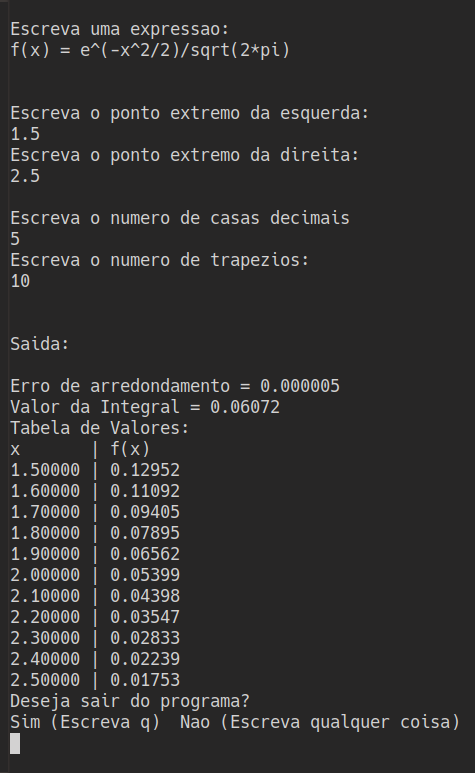
\includegraphics[scale=0.5]{exemplo}
\end{center}

\end{document}
